\section{问题一：确定性购电与储能调度}
\subsection{统一物理模型}
令净负荷电量为$n_t=(L_t-G_t)\Delta t$。供需与SOC递推写为
\begin{align}g_t+q_t-c_t&\ge n_t,\label{eq:balance}\\S_t&=S_{t-1}+\eta_c c_t-q_t/\eta_d.\label{eq:soc}\end{align}
约束为$1200\le S_t\le10800$，$0\le c_t,q_t\le5000/6$，且$S_0=S_{144}=6000$。代码以不等式~\eqref{eq:balance}表示可弃置的富余供给，等价于加入非负弃电变量后写等式。目标函数为
\begin{equation}\min \sum_{t=1}^{144}\pi_tg_t+10^{-7}\sum_{t=1}^{144}(c_t+q_t),\label{eq:q1obj}\end{equation}
其中极小正则项只用于排除退化的同时充放电，不改变两位小数费用结论。模型由HiGHS线性规划求解；其底层高性能对偶修正单纯形方法见文献\textsuperscript{[3]}。求解后独立回代供需、SOC和充放电互斥。
\subsection{结果与基线比较}
主模型购电费为35,126.95元，全天购电59,482.70 kWh；无储能直接购电基线为48,052.05元，节省26.90\%。储能充电20,740.67 kWh、放电16,799.94 kWh，SOC由6,000 kWh回到6,000 kWh，且始终位于1,200--10,800 kWh。图~\ref{fig:q1dispatch}表明，储能在低价或光伏富余时段吸收电量，并在高价时段释放。
\begin{figure}[H]\centering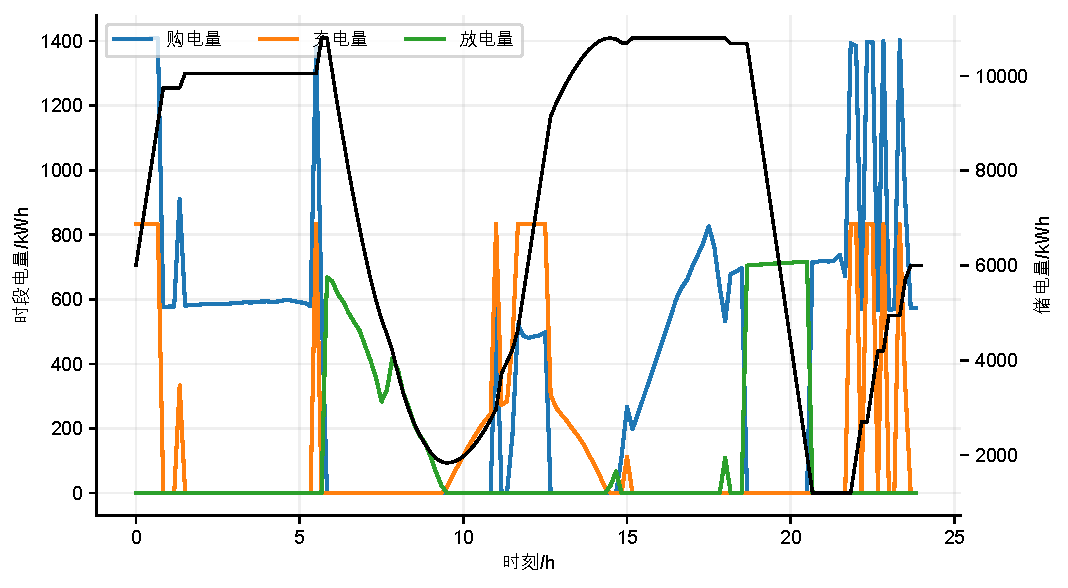
\includegraphics[width=0.94\textwidth]{../figures/fig02_q1_dispatch.pdf}
\caption{问题一购电、充放电与SOC轨迹}\label{fig:q1dispatch}\end{figure}
